\chapter{Исследовательская часть}

В данном разделе будут приведены примеры работы программ, постановка эксперимента и сравнительный анализ алгоритмов на основе полученных данных.

\section{Технические характеристики}
Тестирование выполнялось на устройстве со следующими техническими характеристиками:
\begin{itemize}
	\item Операционная система Pop!\_OS 22.04 LTS \cite{ubuntu} Linux \cite{linux};
	\item Оперативная память 16 Гб;
	\item Процессор AMD® Ryzen 7 2700 eight-core processor × 16 \cite{amd}.
\end{itemize}
Во время тестирования устройство было подключено к блоку питания и не нагружено никакими приложениями, кроме встроенных приложений окружения, окружением и системой тестирования.

\section{Демонстрация работы программы}

Программа получает на вход 2 слова и выдает 4 расстояния, соответствующих алгоритмов поиска редакторского расстояния Левенштейна, итеративного Дамерау-Левенштейна, рекурсивного Дамерау-Левентейна, рекурсивного с мемоизацией Дамерау-Левенштейна.

На рисунке \ref{demonstration} представлен результат работы программы.

\begin{figure}[ht!]
	\begin{center}
		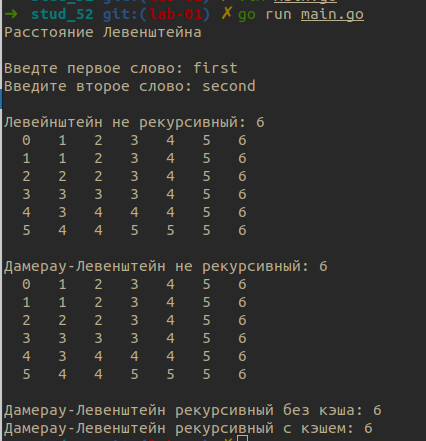
\includegraphics[]{assets/demonst.png}
	\end{center}
	
	\caption{Пример работы программы}
	\label{demonstration}
\end{figure}

\newpage

\section{Время выполнения алгоритмов}

Алгоритмы тестировались при помощи профилирования --- сбора характеристик работы программы: времени выполнения. Для каждой функции были написаны тесты оценки эффективности, представленные библиотеками Си.

\newpage

\begin{lstlisting}[label=bench,caption=Пример теста эффективности]
import "C"	

func test(){
	
	cputime1 := C.getThreadCpuTimeNs()
	
	doWork()
	
	cputime2 := C.getThreadCpuTimeNs()
	fmt.Printf(cputime2 - cputime1)
	
}
\end{lstlisting}

Результаты тестирования приведены в таблице. Прочерк в таблице означает что тестирование для этого набора данных не выполнялось.

\begin{table}[ht!]
	\begin{center}
		\caption{Время выполнения алгоритмов}
		\begin{tabular}{ ||p{1.5cm}||p{2cm}|p{2cm}|p{2cm}|p{3.5cm}||  }
			\hline
			\multirow{2}{*}{Длина}& \multicolumn{4}{c||}{Время выполнения} \\[1.5ex]
			\cline{2-5} 
			строк& ДЛ (кэш)  & ДЛ (итер.) & Лев (итер.) & ДЛ (рек.) \\ [1.5ex] 
			\hline\hline
			5  & 2344 & 1114 & 1091 & 17228 \\
			10 & 6747 & 3142 & 2823 & 109170295 \\
			40 & 92218 & 36281 & 33362 &  - \\
			80 & 402839 & 142910 & 122148 & - \\
			160 & 1582974 & 646498 & 499268 & - \\
			240 & 3505394 & 1348110 & 1122182 & - \\
			\hline
		\end{tabular}
		\label{time-table}
	\end{center}
\end{table}

\newpage

\begin{figure}[ht!]
	\begin{center}
		\begin{tikzpicture}
			\begin{axis}[
				legend pos = north west,
				xlabel=длина строки,
				ylabel=наносекунды,
				minor tick num = 1,
				grid = both,
				major grid style = {lightgray},
				minor grid style = {lightgray!25},
				xtick distance = 40,
				width = 0.9\textwidth,
				height = 0.7\textwidth]
				
				\addplot[
				red,
				semithick,
				mark = *,
				] file {assets/d-lev-mem.dat};
				
				\addplot[
				blue,
				semithick,
				mark = x,
				mark size = 3pt,
				thick,
				] file {assets/d-lev-iter-perf.dat};	
				
				\addplot[
				green,
				semithick,
				mark = *,
				] file {assets/d-lev-recursive.dat};
				
				\legend{
					мемоизацией,
					итеративного,
					рекурсивного,
				}
			\end{axis}
		\end{tikzpicture}
	\end{center}
	\caption{Сравнение рекурсивного с мемоизацией, итеративного и рекурсивного расстояния Дамерау\,--\,Левенштейна}
\end{figure}

\newpage

\begin{figure}[ht!]
	\begin{center}
		\begin{tikzpicture}
			\begin{axis}[
				legend pos = north west,
				xlabel=длина строки,
				ylabel=наносекунды,
				minor tick num = 1,
				grid = both,
				major grid style = {lightgray},
				minor grid style = {lightgray!25},
				xtick distance = 40,
				width = 0.9\textwidth,
				height = 0.7\textwidth]
				
				\addplot[
				red,
				semithick,
				mark = *,
				] file {assets/d-lev-mem.dat};
				
				\addplot[
				blue,
				semithick,
				mark = x,
				mark size = 3pt,
				thick,
				] file {assets/d-lev-iter-perf.dat};
				
				\legend{
					мемоизацией,
					итеративного,
				}
			\end{axis}
		\end{tikzpicture}
	\end{center}
	\caption{Сравнение рекурсивного с мемоизацией, итеративного расстояния Дамерау\,--\,Левенштейна}
\end{figure}



\section{Использование памяти}

Далее будем считать, что $sizeof(int) = 8$, $sizeof(char) = 1$, $sizeof(slice) = 24$. Все значения в этом разделе указываются в байтах.

Длину строки $S_1$ обозначим как n, а длину строки $S_2$ --- как m. Тогда затраченную память можно вычислить следующим образом:

\subsection{Нерекурсивный алгоритм поиска расстояния Дамерау-Левенштейна}
Размер выделяемой памяти:
\begin{itemize}
	\item размер строк $S_1$, $S_2$ --- $m + n$;
	\item размер n = $2$ и m = $8$;
	\item размер матрицы --- $8 \cdot (m + 1) \cdot (n + 1)$;
	\item размер вспомогательных переменных в циклах --- $8 + 8 + 6 \cdot 8$.
\end{itemize}
Таким образом, общая затраченная память в нерекурсивном алгоритме равняется $8mn + 9m + 9n + 88$


\subsection{Рекурсивный алгоритм поиска расстояния без кэша Дамерау-Левенштейна}
Максимальная глубина стека вызовов при рекурсивной реализации равна сумме длин входящий строк.

Размер общей выделяемой памяти:
\begin{itemize}
	\item размер строк $S_1$, $S_2$ --- $m + n$;
	\item размер n = $2$ и m = $8$.
\end{itemize}

Размер выделяемой памяти для каждого вызова функции:
\begin{itemize}
	\item размер аргументов функции --- $2 \cdot 24 + 2 \cdot 8$;
	\item размер вспомогательных переменных --- $6 \cdot 8$;
	\item размер адреса возврата --- $4$.
\end{itemize}
Таким образом, общая затраченная память в рекурсивном алгоритме равняется $m + n + 2 \cdot 8 + (2 \cdot 24 + 2 \cdot 8 + 6 \cdot 8 + 4) \cdot (n + m) = 117m + 117n + 16$

\subsection{Рекурсивный алгоритм поиска расстояния с использованием кэша Дамерау-Левенштейна}
Максимальная глубина стека вызовов при рекурсивной реализации равна сумме длин входящий строк.

Размер общей выделяемой памяти:
\begin{itemize}
	\item размер строк $S_1$, $S_2$ --- $m + n$;
	\item размер n = $2$ и m = $8$;
	\item размер матрицы --- $8 \cdot (m + 1) \cdot (n + 1)$.
\end{itemize}

Размер выделяемой памяти для каждого вызова функции:
\begin{itemize}
	\item размер аргументов функции --- $3 \cdot 24 + 2 \cdot 8$;
	\item размер вспомогательных переменных --- $6 \cdot 8$;
	\item размер адреса возврата --- $4$.
\end{itemize}
Таким образом, общая затраченная память в рекурсивном алгоритме равняется $m + n + 2 \cdot 8 + 8 \cdot (m + 1) \cdot (n + 1) + (3 \cdot 24 + 2 \cdot 8 + 6 \cdot 8 + 4) \cdot (n + m) = 8mn + 149m + 149n + 24$


\section{Вывод}
В данном разделе были сравнены алгоритмы по памяти и по времени.
Рекурсивный алгоритм  Дамерау\,--\,Левенштейна работает дольше итеративных реализаций --- время этого алгоритма увеличивается в геометрической прогрессии с ростом размера строк.
Рекурсивный алгоритм с мемоизацией превосходит простой рекурсивный алгоритм по времени. 
По расходу памяти все реализации проигрывают рекурсивной за счет большого количества выделенной памяти под матрицу расстояний. 

То есть самым эффективный по памяти: рекурсивный алгоритм.
Самый эффективный по времени: итеративный алгоритм (исходя из сделанных тестов.)  

Стоит отметить, что для языков, где возможна передача указателя на массивы, самым эффективным и по времени, и по памяти будет алгоритм, использующий мемоизацию.